\documentclass{article}
\usepackage{color}
\usepackage{tikz}
\usepackage{ntheorem}
\theoremseparator{:}
\newtheorem{hyp}{Hypothesis}
\usetikzlibrary{shapes,decorations,arrows,calc,arrows.meta,fit,positioning}
\tikzset{
    -Latex,auto,node distance =1 cm and 1 cm,semithick,
    state/.style ={ellipse, draw, minimum width = 0.7 cm},
    point/.style = {circle, draw, inner sep=0.04cm,fill,node contents={}},
    bidirected/.style={Latex-Latex,dashed},
    el/.style = {inner sep=2pt, align=left, sloped}
}

\begin{document}
\section{Data Prep, EDA, and Theory development}
\subsection{Varaible Selection \& Explanation}
\indent For the purpose of analyzing the determinats of house (sales) prices in the US a theory was developed based on combining two common valuation strategies in real-estate; "vergleichswert verfahren, sachwert verfahren".

\indent Based on the theory, four categories of regressors were identified in the data, promising to best represent the population regression equation. 
\begin{itemize}
  \item Size related quantities (House size, lot size); garage
  \item District and Neighborhood dependent variables; Zoning
  \item type of housing (one family home, apartment, etc)
  \item Quality and condition of the house; including time since remodeling
\end{itemize}

\textbf{NOTE: WHY DO YOU MERGE ZONING? OR HOUSING?}

To this end, this reasearch assignemnt draws data from an apprisal project conducted by... in the Ames district, Iowa (USA) (CITE DATA SOURCE HERE!!!). Corresponding to the aforementioned data categories, the following variables were selected to be used in varying degrees in the model. It may be noted, that due to the data being limited to a city in the midwest of the USA, the generalization resulting from this research may only extend to similar cities. However, due to the data originating from one district alone results in the comparability of the sale instances recorded in the data; meaning that stark contrasts in sales prices may be less due to the simple fact that one sale may have been made in Iowa and the other in New York, which naturally yields higher prices.
\textbf{INCLUDE FREQQUENCY TABLES FOR THE CATEGORICAL VAIRABLES}

\textbf{Preanalysis: is quality as an interval? IMPORTANT: ARGUE WHY WE THING THAT QUALITY IS AN INTERVAL HERE LIKE LIKERT SCALE?!?!!?!}
%#' arguemtns for quality being a numeric variable:
%#' 1. like a likert scale
%#' 2. the standard errors are extremely constant
%#' 3. The plot suggests the same
%#' 4. the estimates increase steadily´
%#' PLOT IT!




To start, a total of 1,460 house sales were recorded between 2006 and 2010 for the district of Ames, Iowa (USA). The dependent varibale was identified to be SalePrice. As can be observed in Table 1, the mean sale price of a house was \$180,921.20 (SD = 79,442.50). Combined with the range [34,900, 755,000] a positive skewness was to be expected (skew = 1.881), considering that the outcome variable is a of financial nature.
\textbf{IMPORTANT! TELL THAT WE HAVE LARGE RANGES ETC SO THIS MEAN WE NEED STANDARDIZED COEF}

\indent Following, the first category of data pertains to size related dimensions of the property sold. More specifically, the total living area (tot\_living\_area)\footnote{defined as summing above- and below- ground or base living.} displays a mean of 2,572.89 square feet (SD = 823.598) in addition to a large reange of values[334, 11,752]; suggesting that the sales were conducted in neighborhoods (Neighborhood) included range from urban to (partially) rural. To this end, the second data category encompasses the zoning classification (MSZoning) which identifies neighborhoods and the correpsonding sales as rural or not. Neighborhood consisists of 25 distinctions and zoning of eight categories\footnote{only 5 categories actually contain data.}, which will be adjusted to three categories to decrease the complexity of the data analysis (see Appendix for a contignecy table). Additionally, the number of bedrooms above ground level (mean = 2.866, SD = 0.816) (BedroomAbvGr) and the number of bathrooms (mean = 1.990, SD = 0.732) are included (tot\_bathrooms)\footnote{The correlation betwen house size and number of bedrooms and bathrooms will be addressed later}. 
\indent Moreover, the third class of data was selected to balance size and neighborhood related associations by consideringh building type (BldgType), which consists of five categories. Interestingly, the majority of sold homes were one-family homes (n = 1220); this variable was adjusted to reduce the complexity of the data analysis and remove confusion about the definition of building type.
\indent The fourth category contains quality and condition related variables. Both variables are on a discrete  scale from one to ten. Quality displays values for each quality rating (mean = 6.099, SD = 1.383), while the condition ranges from one to nine (mean = 5.575, SD = 1.113).

\textbf{TIME SINCE REMODELING AT YEAR OF SALE; Time since building is also negative but this one is clearer!; ALSO THIS RELATIPONSHIP HOLDS FOR NEIGHBORHOODS!!!!}
 

% Table created by stargazer v.5.2.3 by Marek Hlavac, Social Policy Institute. E-mail: marek.hlavac at gmail.com
% Date and time: Fri, Sep 09, 2022 - 22:51:21
\begin{center}
\begin{table}[!htbp] \centering 
  \caption{Descriptive Statistics} 
  \label{} 
\begin{tabular}{@{\extracolsep{5pt}}lccccc} 
\\[-1.8ex]\hline 
\hline \\[-1.8ex] 
Statistic & \multicolumn{1}{c}{N} & \multicolumn{1}{c}{Mean} & \multicolumn{1}{c}{St. Dev.} & \multicolumn{1}{c}{Min} & \multicolumn{1}{c}{Max} \\ 
\hline \\[-1.8ex] 
SalePrice & 1,460 & 180,921.200 & 79,442.500 & 34,900 & 755,000 \\ 
YearBuilt & 1,460 & 1,971.268 & 30.203 & 1,872 & 2,010 \\ 
YearRemodAdd & 1,460 & 1,984.866 & 20.645 & 1,950 & 2,010 \\ 
LotArea & 1,460 & 10,516.830 & 9,981.265 & 1,300 & 215,245 \\ 
GrLivArea & 1,460 & 1,515.464 & 525.480 & 334 & 5,642 \\ 
TotalBsmtSF & 1,460 & 1,057.429 & 438.705 & 0 & 6,110 \\ 
BedroomAbvGr & 1,460 & 2.866 & 0.816 & 0 & 8 \\ 
BsmtFullBath & 1,460 & 0.425 & 0.519 & 0 & 3 \\ 
FullBath & 1,460 & 1.565 & 0.551 & 0 & 3 \\ 
PoolArea & 1,460 & 0.005 & 0.069 & 0 & 1 \\ 
GarageCars & 1,460 & 1.767 & 0.747 & 0 & 4 \\ 
OverallQual & 1,460 & 6.099 & 1.383 & 1 & 10 \\ 
OverallCond & 1,460 & 5.575 & 1.113 & 1 & 9 \\ 
tot\_living\_area & 1,460 & 2,572.893 & 823.598 & 334 & 11,752 \\ 
tot\_bathrooms & 1,460 & 1.990 & 0.732 & 0 & 6 \\ 
Adjacent\_features\_bool & 1,460 & 0.137 & 0.344 & 0 & 1 \\ 
\hline \\[-1.8ex] 
\end{tabular} 
\end{table} 
\end{center}

\textbf{KEEP STAT PART IN STARGAZER USE QUANTILES IN THE SUMMARY STATISTIC; ANd remove the N; ALSO ADD DESCRIPTIVES}

It is notable that upon selecting the aforementioned variables, no preprossessing in the form of imputation or data deletion had to be applied. However, in order to decrease the complecity of the interaction term, the variable MSZoning was binned into (rural, mixed rural, and urban) based on the corresponding zoning categories\footnote{$https://www.kaggle.com/competitions/home-data-for-ml-course/data$}.


\subsection{Exploratory Data Analysis}\footnote{The theory underlying the choice of the variables will be further elaborated upon in Section 2}
A scatter plot matrix is provided in the appendix for the numeric variables. The EDA shows the four data categories with respect to the sale price of the property. Thus, the plots represented, inter alia, drove the development of the hypothesis down the line in combination with the aforementioned valuation strategies. 

\section{Theoretical model and OLS assumptions}




\begin{center}
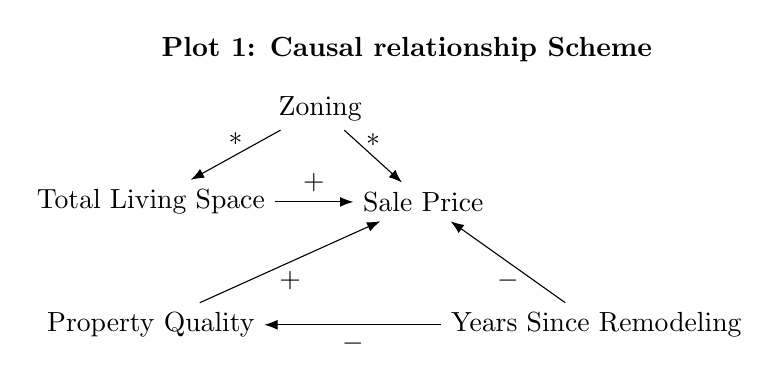
\begin{tikzpicture}
	\centering
 	\node at (3.25,3.5) {\textbf{Plot 1: Causal relationship Scheme}};
    \node (1) at (0,0) {Property Quality};
	\node (2) [above = of 1] {Total Living Space};
	\node (3) [right = of 2] {Sale Price};
	\node (4) at (2.15,2.75) {Zoning};
	\node (5) [right = of 1] {};
	%\node (6) [right = of 4] {LotArea};
	\node (7) [right = of 5] {Years Since Remodeling};
	

	%\path (1) edge node[left] {$?$} (7);
	\path (7) edge node[below] {$-$} (1);
	\path (7) edge node[below] {$-$} (3);
	\path (1) edge node[below] {$+$} (3);
	\path (2) edge node[above] {$+$} (3);
	\path (4) edge node[above] {$*$} (2);
	%\path (4) edge node[above] {$*$} (6);
	\path (4) edge node[above] {$*$} (3);
%	\path (6) edge node[right] {$+$} (3);
	
\end{tikzpicture}
\end{center}

$$ {SalePrice} = \alpha + \beta_{1} TotalLivingSpace - \beta_{2}  Property Quality - \beta_{3}  YearsSinceRemodeling  \linebreak
+ \beta_{4}  LotArea + \beta_{5} Zoning + \epsilon$$


\indent Based on the valuation strategies and EDA discussed above, a theory was set up to explain the variation in sales prices. The corresponding causal relationship scheme can be seen in Plot 1. 

\indent \paragraph{} \textbf{Plot XXX} displays a potential direct positive association between Total Living Space (IV) and Sale Price (DV). Thus, one expects that larger houses have a higher sale price. Consequently,we assume that:

\begin{hyp}[H\ref{hyp:first}] \label{hyp:first}
Total living space (IV) has a direct postive association with Sales Price (DV)
\end{hyp}

\begin{center}
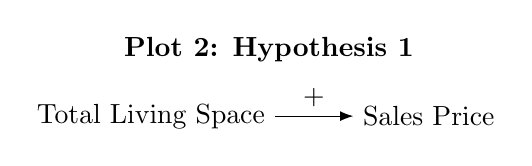
\begin{tikzpicture}
	\centering
 	\node at (1.5,0.85) {\textbf{Plot 2: Hypothesis 1}};
 	\node (1) at (0,0) {Total Living Space};
	\node (2) [right = of 1] {Sales Price};
	\path (1) edge node[above] {$+$}(2);
\end{tikzpicture}
\end{center}


\indent \paragraph{} Subsequently, when taking the Zoning (MSZoning or MSZoning\_grouped - IV) into account to reflect the administrative borderrs of the Ames districts, larger houses in more densly populated areas of the city appear to have a lower price when compared to houses of same size in less densly populated areas as can be seen in \textbf{Plot XXXX2}. This suggests a separation between "downtown less affluent areas" and "suburban affluent areas"\footnote{As an extention\: we will test whether the groups of Neighborhoods generally stay in the same zoning category; if Neighborhoods and Zoning are not related (so eg 50 \% of one neighborhood is in rural zone while the other part is in moderately populated zone) then we have a problem that this woudl induce a bias. Otherwise, we can just proceed.} and concludes in the hypothesis that

\begin{hyp}[H\ref{hyp:second}] \label{hyp:second}
Zoning moderates (MIV) the direct postive association of Total Living Space (IV) and Sale Price (DV). The association of Space and Sale Price is proposed to be weaker for more densly populated areas than for more rural areas. 
\end{hyp}

\begin{center}
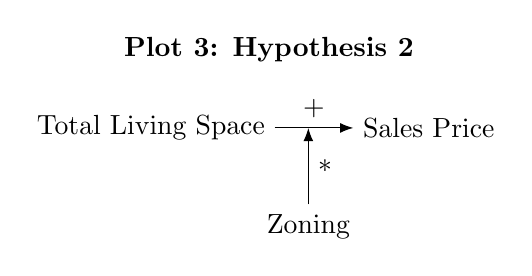
\begin{tikzpicture}
	\centering
 	\node at (1.5,1) {\textbf{Plot 3: Hypothesis 2}};
 	\node (1) at (0,0) {Total Living Space};
	\node (2) [right = of 1] {Sales Price};
	\node (3) at (2,-1.25) {Zoning};
	
	\coordinate (4) at (2,0);
	
	\path (1) edge node[above] {$+$}(2);
	\path (3) edge node[right] {$*$}(4);
\end{tikzpicture}
\end{center}


\indent \paragraph{} Finally, the sales price is not only dependent on the size and the location of the construction, but also its Quality (IV). Correspondingly, one might assume a positive relationship between the quality of a given property and the Years Since Remodeling (M-IV) or Construction. Thus, the final hypothesis states that\footnote{Note that in order for this hypothesis to work, an initial association of Years Since Remodeling would have to be included in previous Hypotheses}
\begin{hyp}[H\ref{hyp:third}] \label{hyp:third}
Years Since Remodeling (M-IV) or Construction has an amplyfiying effect on the direct postive effect of Quality (IV) and Sale Price (DV)
\end{hyp}

\begin{center}
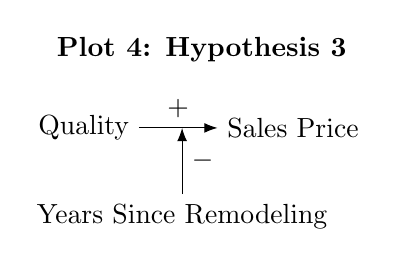
\begin{tikzpicture}
	\centering
 	\node at (1.5,1) {\textbf{Plot 4: Hypothesis 3}};
 	\node (1) at (0,0) {Quality};
	\node (2) [right = of 1] {Sales Price};
	\node (3) at (1.25,-1.12) {Years Since Remodeling};
	
	\coordinate (4) at (1.25,0);
	\path (1) edge node[above] {$+$}(2);
	\path (3) edge node[right] {$-$}(4);
\end{tikzpicture}
\end{center}


%$$ {SalePrice} = \alpha + \beta_{1} TotLivingSpace - \beta_{2}  TotLivingSpace^2 + \beta_{3}  Quality + \beta_{4}  Zoning_{Low Density} + \beta_{5}  Zoning_{Other} + \beta_{6}  YearsSinceRemodeling + \beta_{7}  LotArea + \beta_{8} TotLivingSpace*Zoning_{Low Density} + \beta_{9} TotLivingSpace*Zoning_{Other} +\epsilon$$



\textbf{IMPORTANT: DO YOU INCLUDE A QUADRATIC TERM IN THE POPULATION REGRESSION MODEL???? NO! BUt make more equations explaining each quadartic term and represent the interaction effects etc adn what not }

%$$ {SalePrice} = \alpha + \beta_{1} TotLivingSpace - \beta_{2}  TotLivingSpace^2 + \beta_{3}  Quality + \beta_{4}  Zoning - \beta_{5}  YearsSinceRemodeling + \beta_{6}  LotArea + \beta_{7} TotLivingSpace*Zoning + \beta_{8} AdjacentFeatures + \beta_{9} BuildingType \epsilon$$





\indent \paragraph{Assumtions for Linear Regression} Considering the population regression model above, the first assumptions requires a linear relationship between the independent and the dependent variables. As could be observed during the EDA in part 1, this assumtion is likely to hold, with a weak nonliear relationship of Total Living Area and Sale Price; this can be rectivfied using a quadratic term. 

https://statisticsbyjim.com/regression/ols-linear-regression-assumptions/

A1: Linearity of model parameters and error term; through the formulation of the (population) regression model, addressing the models' functional form. Thus, a violation of this assumtion is practically impossible if the functional for of the population regression is defined correctly. WHeterh the relationship between the indent and the dependent is of linear nature.
The linearity of model parameters and error term assumption suggests that a) the functional form of the underlying population regression model is linear and additive. Additionally, the explanatory variables have to be linearly associated with the dependent. This assumption is easily violated. As can be seen in \textbf{plot xxx and the corresponding appendix with the best fitted line}, Total Living Space displayes a slight quadratic relationship with the Sale Price. the reason why this might be the case may be that with increasion values for x ([X = x]), the effect of X on Y increases, which would be represented in later regression models by an additional quadratic term in the regression equation. However, as will be shown in later parts, this can be (partially) remedied.


A2: desribes that for a linear system to be solvable, no independent variable can be a linear function of other independent variables; e.g. this way a 2-dimensional sphere might be compressed to a line, figuratively speaking, meaning that there is no optimal (or none at all) solution for the parameters in question. This first part of the assumtion might easily be violated when not dropping a "comparative" category of a categorical varaible. However, violations of full rank might also come in the form of multicollinearity. Multicollinearity is the "almost" violation of the full rank violation as a given variable may, for isntance, be highly correlated with another given variable. This way the sphere is almost compressed to a single line, which leads to a multitute of problems regarding inference of the model: primairly, the standard errors of the model become unstable to the inclusion of other explanatory or control variables. This assumption is commonly to some extend violated, as some multicollinearity is always present between the explanatory variables (actually making regression interesting in the first place). As such, a good example might be if we included the Total Linving Space and the TotalNumberofRooms, both of which will be strongly correlated. Further tests will be conducted to probe for this assumption violation. 

A3: This assumption is referred to as mean independence (or exogeniety); assuming no correlation/systematic association between independent variables and residuals (or conditional mean error is dependent on independent variables). Thus this assumption might induce a bais/ or reduce consistency of the estimator and is, thus, critical to the model itself. A common way, this variable is violated is via unobserved confounders or ommitted variables. If a given variable is left out, part of the error term can be explained by a given variable which suffers under the influence of the confounder. An example in this case will be the missign information regariding crime by neighborhood. It is obvious that higher crime levels will reduce the value in a given area. Thus, given a certain Neighborhood in question, part of the variance that would have been explained by the Crime variable is now falsely attributed to Neighborhood, biasing the estimate.

A4: The error term has a constant variance for each observation expected! --> heteroscedasticity
The assumption of homoscedasticity suggests constance variance of each observation. However, if the variance of the estimate is varying we face heteroscedastic variances. While this is not necessarily problematic regarding the estimated parameter (coefficient), heteroscedastictiy impacts the standard errors of the estimate, leading to problems regarding inference; heteroscedastitiy can lead to both type I and II error. In this research, this violation might occur if the eg. sales prices vary stronger for large houses than for small houses. The resulting (averaged) standard error would neither be rebresenative for small and large house standard errors and, thus, inference itself.


Generally, as the sample size increases, this assumption becomes less important for the estimate itself, considering that OLS is a consistent estimator; which is the case here (N is quite large). However, heteroscedastictiy may lead to problems regarding inference, as the standard error of the estimate may still be biased. As such, solutions will be later implemented to control for such violations.

\textbf{DISUSS WHAT CAN GO WRONG APPLIED TO MY DATA AND MY MODEL like last lecture in eci; Come up with a situation where this is violated; EG FULL RANK: NUMBER OF BEDROOMS AND TOTAL LIVING SPACE; HOUSE SIZE AND TOTAL LOT SIZE can pose multicollinearity problems}

A5: Data generation: xi can be random or fixed; the data was collected for predictive purposes so we might not be able to veryfy this. 

A6: This assumption regards inference; if the residuals do not follow a standard normal distribution, this might result in incorrect decisions as the distribution might for instance be "fatter" in the tails, resulting in potentially Type I or Type II errors. This might be the case if for instance we do not have a lot of observations for e.g. subcategories. Subsequently, the resulting inference might be biased. However, as the sample size increases, most distributions approach the normal form. 

Normal distribution of disturbanc (The error term is normally distributed. generally, the means that the error term has a population mean of zeor and standard errror of 1. Generally, most distributions tend to approach normal distributions as sample sizes increase. For some distirbutions such as Sales Price (which is of a financial nature), this can also be remedied through tra´nsforming (here apply log transform). Additionally, multiple controls and test will be conducted down the line to investiate this issue.






\section{OLS regression and model fit}




























The study of Sales Price of property in Ames, Iowa, has shown that the Total Living Area has a significant postive effect on the Sales Price ($\hat{\beta}$ = 0.040, $p$ = 0.01)

\paragraph{Effect Size} regarding teh discussion which variable has the largest effect sized, the standardized coefficietns were used. This is primarily due to the large ranges in some varaibles such as total living area [334, 11,752] when compared to Quality [1,10]. This will cause the OLS to overstate the the cofificent with the large range in values, amking it appear to be greater than it is. Thus, to this end we use standardized coefficients

% Table created by stargazer v.5.2.3 by Marek Hlavac, Social Policy Institute. E-mail: marek.hlavac at gmail.com
% Date and time: Tue, Sep 13, 2022 - 11:19:41
\begin{table}[!htbp] \centering 
  \caption{Unstandardized Coefficinets} 
  \label{Unstandardized Coefficinets} 
\begin{tabular}{@{\extracolsep{5pt}}lccc} 
\\[-1.8ex]\hline 
\hline \\[-1.8ex] 
 & \multicolumn{3}{c}{\textit{Dependent variable:}} \\ 
\cline{2-4} 
\\[-1.8ex] & \multicolumn{3}{c}{SalePrice} \\ 
\\[-1.8ex] & (1) & (2) & (3)\\ 
\hline \\[-1.8ex] 
 tot\_liv\_area & 0.075$^{***}$ & 0.042$^{***}$ & 0.056$^{***}$ \\ 
  & (0.002) & (0.002) & (0.004) \\ 
  & & & \\ 
 I(tot\_liv\_area$\hat{\mkern6mu}$2) &  &  & $-$0.00000$^{***}$ \\ 
  &  &  & (0.00000) \\ 
  & & & \\ 
 OverallQual &  & 23.991$^{***}$ & 31.638$^{***}$ \\ 
  &  & (1.125) & (1.266) \\ 
  & & & \\ 
 low\_density\_zone &  & 19.720$^{***}$ & $-$23.347$^{***}$ \\ 
  &  & (2.897) & (9.011) \\ 
  & & & \\ 
 other\_zone &  & 12.487$^{**}$ & $-$63.223$^{***}$ \\ 
  &  & (5.336) & (20.282) \\ 
  & & & \\ 
 y\_since\_rem &  & $-$0.445$^{***}$ & 2.274$^{***}$ \\ 
  &  & (0.060) & (0.219) \\ 
  & & & \\ 
 LotArea &  &  & 0.001$^{***}$ \\ 
  &  &  & (0.0001) \\ 
  & & & \\ 
 OverallQual:y\_since\_rem &  &  & $-$0.487$^{***}$ \\ 
  &  &  & (0.038) \\ 
  & & & \\ 
 tot\_liv\_area:low\_density\_zone &  &  & 0.017$^{***}$ \\ 
  &  &  & (0.004) \\ 
  & & & \\ 
 tot\_liv\_area:other\_zone &  &  & 0.028$^{***}$ \\ 
  &  &  & (0.008) \\ 
  & & & \\ 
 Constant & $-$12.397$^{***}$ & $-$80.656$^{***}$ & $-$137.445$^{***}$ \\ 
  & (4.279) & (6.599) & (10.840) \\ 
  & & & \\ 
\hline \\[-1.8ex] 
Observations & 1,460 & 1,460 & 1,460 \\ 
R$^{2}$ & 0.607 & 0.758 & 0.799 \\ 
Adjusted R$^{2}$ & 0.607 & 0.758 & 0.798 \\ 
Residual Std. Error & 49.833 (df = 1458) & 39.107 (df = 1454) & 35.744 (df = 1449) \\ 
F Statistic & 2,249.818$^{***}$  & 913.326$^{***}$  & 575.803$^{***}$  \\ 
 & (df = 1; 1458) & (df = 5; 1454) & (df = 10; 1449) \\
\hline 
\hline \\[-1.8ex] 
\textit{Note:}  & \multicolumn{3}{r}{$^{*}$p$<$0.1; $^{**}$p$<$0.05; $^{***}$p$<$0.01} \\ 
\end{tabular} 
\end{table}




% Table created by stargazer v.5.2.3 by Marek Hlavac, Social Policy Institute. E-mail: marek.hlavac at gmail.com
% Date and time: Tue, Sep 13, 2022 - 11:34:56
\begin{table}[!htbp] \centering 
  \caption{Scale Independent Varaibles AND outcome variable} 
  \label{Scale Independent Varaibles AND outcome variable} 
\begin{tabular}{@{\extracolsep{5pt}}lccc} 
\\[-1.8ex]\hline 
\hline \\[-1.8ex] 
 & \multicolumn{3}{c}{\textit{Dependent variable:}} \\ 
\cline{2-4} 
\\[-1.8ex] & \multicolumn{3}{c}{scale(SalePrice)} \\ 
\\[-1.8ex] & (1) & (2) & (3)\\ 
\hline \\[-1.8ex] 
 scale(tot\_liv\_area) & 0.779$^{***}$ & 0.440$^{***}$ & 0.513$^{***}$ \\ 
  & (0.016) & (0.018) & (0.019) \\ 
  & & & \\ 
 scale(OverallQual) &  & 0.418$^{***}$ & 0.346$^{***}$ \\ 
  &  & (0.020) & (0.019) \\ 
  & & & \\ 
 scale(low\_density\_zone) &  & 0.101$^{***}$ & 0.115$^{***}$ \\ 
  &  & (0.015) & (0.016) \\ 
  & & & \\ 
 scale(other\_zone) &  & 0.035$^{**}$ & 0.026$^{*}$ \\ 
  &  & (0.015) & (0.015) \\ 
  & & & \\ 
 scale(y\_since\_rem) &  & $-$0.116$^{***}$ & $-$0.174$^{***}$ \\ 
  &  & (0.016) & (0.016) \\ 
  & & & \\ 
 I(scale(tot\_liv\_area)$\hat{\mkern6mu}$2) &  &  & $-$0.038$^{***}$ \\ 
  &  &  & (0.004) \\ 
  & & & \\ 
 scale(tot\_liv\_area):scale(low\_density\_zone) &  &  & 0.074$^{***}$ \\ 
  &  &  & (0.017) \\ 
  & & & \\ 
 scale(tot\_liv\_area):scale(other\_zone) &  &  & 0.065$^{***}$ \\ 
  &  &  & (0.019) \\ 
  & & & \\ 
 scale(OverallQual):scale(y\_since\_rem) &  &  & $-$0.170$^{***}$ \\ 
  &  &  & (0.014) \\ 
  & & & \\ 
 Constant & 0.000 & 0.000 & $-$0.070$^{***}$ \\ 
  & (0.016) & (0.013) & (0.015) \\ 
  & & & \\ 
\hline \\[-1.8ex] 
Observations & 1,460 & 1,460 & 1,460 \\ 
R$^{2}$ & 0.607 & 0.758 & 0.792 \\ 
Adjusted R$^{2}$ & 0.607 & 0.758 & 0.791 \\ 
Residual Std. Error & 0.627 (df = 1458) & 0.492 (df = 1454) & 0.457 (df = 1450) \\ 
F Statistic & 2,249.818$^{***}$  & 913.326$^{***}$  & 615.168$^{***}$  \\ 
 & (df = 1; 1458) & (df = 5; 1454) & (df = 9; 1450) \\
\hline 
\hline \\[-1.8ex] 
\textit{Note:}  & \multicolumn{3}{r}{$^{*}$p$<$0.1; $^{**}$p$<$0.05; $^{***}$p$<$0.01} \\ 
\end{tabular} 
\end{table} 

% Table created by stargazer v.5.2.3 by Marek Hlavac, Social Policy Institute. E-mail: marek.hlavac at gmail.com
% Date and time: Tue, Sep 13, 2022 - 11:54:25
\begin{table}[!htbp] \centering 
  \caption{Scale Independent Varaibles - Unscaled outcome variable} 
  \label{Scale Independent Varaibles - Unscaled outcome variable} 
\begin{tabular}{@{\extracolsep{5pt}}lccc} 
\\[-1.8ex]\hline 
\hline \\[-1.8ex] 
 & \multicolumn{3}{c}{\textit{Dependent variable:}} \\ 
\cline{2-4} 
\\[-1.8ex] & \multicolumn{3}{c}{SalePrice} \\ 
\\[-1.8ex] & (1) & (2) & (3)\\ 
\hline \\[-1.8ex] 
 scale(tot\_liv\_area) & 61.882$^{***}$ & 34.977$^{***}$ & 40.723$^{***}$ \\ 
  & (1.305) & (1.398) & (1.491) \\ 
  & & & \\ 
 scale(OverallQual) &  & 33.180$^{***}$ & 27.450$^{***}$ \\ 
  &  & (1.556) & (1.494) \\ 
  & & & \\ 
 scale(low\_density\_zone) &  & 8.058$^{***}$ & 9.126$^{***}$ \\ 
  &  & (1.184) & (1.261) \\ 
  & & & \\ 
 scale(other\_zone) &  & 2.757$^{**}$ & 2.088$^{*}$ \\ 
  &  & (1.178) & (1.181) \\ 
  & & & \\ 
 scale(y\_since\_rem) &  & $-$9.182$^{***}$ & $-$13.830$^{***}$ \\ 
  &  & (1.240) & (1.232) \\ 
  & & & \\ 
 I(scale(tot\_liv\_area)$\hat{\mkern6mu}$2) &  &  & $-$3.045$^{***}$ \\ 
  &  &  & (0.302) \\ 
  & & & \\ 
 scale(tot\_liv\_area):scale(low\_density\_zone) &  &  & 5.914$^{***}$ \\ 
  &  &  & (1.336) \\ 
  & & & \\ 
 scale(tot\_liv\_area):scale(other\_zone) &  &  & 5.151$^{***}$ \\ 
  &  &  & (1.508) \\ 
  & & & \\ 
 scale(OverallQual):scale(y\_since\_rem) &  &  & $-$13.471$^{***}$ \\ 
  &  &  & (1.104) \\ 
  & & & \\ 
 Constant & 180.921$^{***}$ & 180.921$^{***}$ & 175.341$^{***}$ \\ 
  & (1.304) & (1.023) & (1.157) \\ 
  & & & \\ 
\hline \\[-1.8ex] 
Observations & 1,460 & 1,460 & 1,460 \\ 
R$^{2}$ & 0.607 & 0.758 & 0.792 \\ 
Adjusted R$^{2}$ & 0.607 & 0.758 & 0.791 \\ 
Residual Std. Error & 49.833 (df = 1458) & 39.107 (df = 1454) & 36.304 (df = 1450) \\ 
F Statistic & 2,249.818$^{***}$  & 913.326$^{***}$  & 615.168$^{***}$  \\ 
 & (df = 1; 1458) & (df = 5; 1454) & (df = 9; 1450) \\
\hline 
\hline \\[-1.8ex] 
\textit{Note:}  & \multicolumn{3}{r}{$^{*}$p$<$0.1; $^{**}$p$<$0.05; $^{***}$p$<$0.01} \\ 
\end{tabular} 
\end{table} 

\section{task 5}
TIPP \textbf{run regression once with and once without the dummies to see the effect of the subsample }

\textbf{IMPORTANT! THEY STANDARDIZED BOTH the regressors AND the dependent variable!!! so only show that

Additionally: when reporting these outputs as stargazer; stargazer does not report the standardized error but the normal coefficeints; so you have to change that to standardized coefficients


BUT THE BIG PROBLEM IS: IF YOU REPORT IT VIA STARGAZER SOME EFFECTS MISS THE ***!!!! even when they are significant; and if you normally standrize it each variabel by hand, then the standard errrors change even though they should not: So to do: get the Std coef from eg "full_model_w_interaction.beta" AND THE STANDARD ERRORS from the normal regression "full_model_w_interaction" output}

\end{document}